\begin{figure}[h] 
\centering 
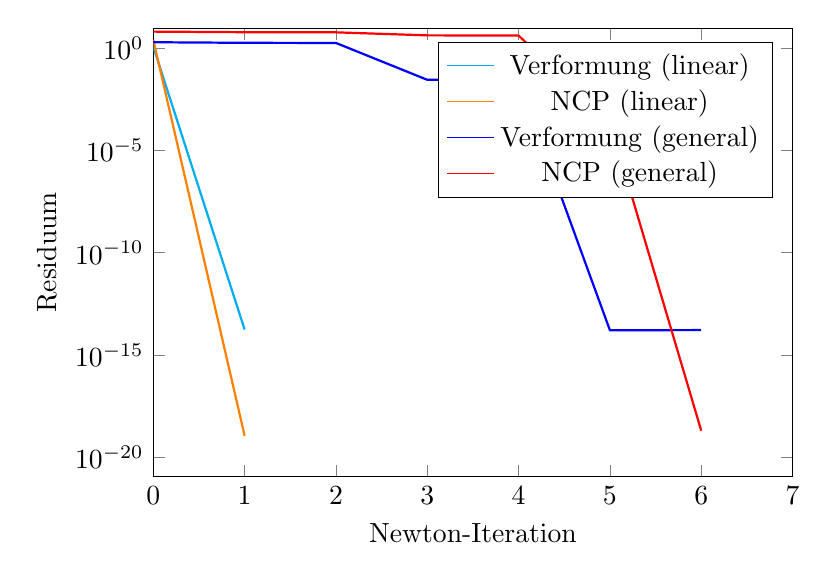
\begin{tikzpicture}[every plot/.append style={thick}] 
\begin{axis}[ 
label style={font=\normalsize}, 
xlabel={Newton-Iteration}, 
ylabel={Residuum}, 
xmin=0, xmax=7, 
ymode=log, 
ymin=0, ymax=10, 
width=0.8\textwidth, 
height=0.6\textwidth, 
legend pos=north east, 
legend style={cells={align=left}}, 
grid style=dashed, 
] 
\addplot[ 
color=cyan, 
] 
coordinates { 
(0, 1.24e+00)(1, 1.73e-14)}; 
\addlegendentry{Verformung (linear)} 
\addplot[ 
color=orange, 
] 
coordinates { 
(0, 2.67e+00)(1, 1.08e-19)}; 
\addlegendentry{NCP (linear)} 
\addplot[ 
color=blue, 
] 
coordinates { 
(0, 2.06e+00)(1, 1.93e+00)(2, 1.90e+00)(3, 2.97e-02)(4, 2.93e-02)(5, 1.60e-14)(6, 1.63e-14)}; 
\addlegendentry{Verformung (general)} 
\addplot[ 
color=red, 
] 
coordinates { 
(0, 6.82e+00)(1, 6.39e+00)(2, 6.29e+00)(3, 4.47e+00)(4, 4.40e+00)(5, 2.47e-04)(6, 1.92e-19)}; 
\addlegendentry{NCP (general)} 
\end{axis} 
\end{tikzpicture} 
\caption{Residuen des Stoffgesetzes 'Linear elastisch' mit Hinderniss 'Hut' und 2178 Freiheitsgraden für die Verschiebung.} 
\label{fiq:Linearelastisch_Hut_level4} 
\end{figure} 
